\documentclass{tufte-handout}

\title{Propositional Probability IV:\\Binary Decision Diagrams\thanks{CS7470 Fall 2023: Foundations of Probabilistic Programming.}}


\newcommand{\varset}[0]{\mathcal{V}}

\author[]{Steven Holtzen\\s.holtzen@northeastern.edu}

%\date{28 March 2010} % without \date command, current date is supplied

%\geometry{showframe} % display margins for debugging page layout
\setcounter{secnumdepth}{1}

\usepackage{graphicx} % allow embedded images
  \setkeys{Gin}{width=\linewidth,totalheight=\textheight,keepaspectratio}
  \graphicspath{{graphics/}} % set of paths to search for images
\usepackage{amsmath,amssymb,amsthm}  % extended mathematics
\usepackage{booktabs} % book-quality tables
\usepackage{units}    % non-stacked fractions and better unit spacing
\usepackage{multicol} % multiple column layout facilities
\usepackage{lipsum}   % filler text
\usepackage{fancyvrb} % extended verbatim environments
  \fvset{fontsize=\normalsize}% default font size for fancy-verbatim environments
\usepackage{listings}
\usepackage{tikz}
\usepackage{mathpartir}
\usepackage{subcaption}
\usepackage{mdframed}
\usepackage{epigraph}
\usepackage{enumitem}
\usepackage{stmaryrd}

\usetikzlibrary{shapes.geometric}


\usepackage[ruled,linesnumbered]{algorithm2e}
\SetKwComment{Comment}{/* }{ */}
\newcommand{\indep}{\perp \!\!\! \perp}

\tikzset{
  treenode/.style = {shape=rectangle, rounded corners,
                     draw, align=center,
                     },
  root/.style     = {treenode, font=\Large, bottom color=red!30},
  env/.style      = {treenode, font=\ttfamily\normalsize},
  dummy/.style    = {circle,draw}
}

% tikz
\usetikzlibrary{patterns,calc,backgrounds}


% TIKZ
\tikzstyle{nnf}=[
  >=stealth,font=\small,auto,scale=0.7,every node/.style={scale=0.7}
]
\tikzstyle{extnode}=[
  draw,circle,inner sep=2pt,fill=white
]

\tikzstyle{leafnode}=[
  draw,fill=gray!20,inner sep=3.5pt
]
\tikzstyle{constnode}=[
  draw,fill=white,inner sep=3.5pt
]
\tikzstyle{label}=[
  fill=white,inner sep=2.5pt
]

\tikzstyle{acarrow}=[
    decoration={markings,mark=at position 1 with {\arrow[scale=0.6]{>}}},
    postaction={decorate},
    shorten >=0.4pt,
    >=latex,
    line width=0.1
]

\tikzstyle{bnarrow}=[
    decoration={markings,mark=at position 1 with {\arrow[scale=1.5]{>}}},
    postaction={decorate},
    shorten >=0.7pt,
    >=latex,
    line width=0.3
]
\tikzstyle{bayesnet}=[
  >=latex, thick, auto
]
\tikzstyle{bnnode}=[
  draw,ellipse,minimum size=7mm,inner sep=1pt,font=\small
]
\tikzstyle{cpt}=[
  font=\footnotesize
]

\tikzstyle{graph}=[
  >=stealth,font=\small,auto,scale=1,every node/.style={scale=1}
]
\tikzstyle{node}=[
  draw,circle,inner sep=3pt,fill=white
]

% BDDs

\tikzstyle{bdd}=[
  >=latex, thick, >=stealth, font=\small,auto,scale=0.9,every node/.style={scale=0.9}
]
\tikzstyle{bddnode}=[
  draw,circle,inner sep=0pt,fill=white,minimum size=5.5mm
]

\tikzstyle{bddtriangle}=[
  draw, regular polygon, regular polygon sides = 3,inner sep=1pt,fill=white,minimum size=5.5mm
]

\tikzstyle{highedge}=[
    line width=0.9
]
\tikzstyle{lowedge}=[
    line width=0.9,dotted
]
\tikzstyle{bddterminal}=[
  draw,fill=gray!20,inner sep=2.5pt, font=\small
]

\lstdefinestyle{compact}{
  \ttfamily\tiny
}


\usetikzlibrary{positioning}

\newtheorem{theorem}{Theorem}
\newtheorem{definition}{Definition}
\newtheorem{conjecture}{Conjecture}
\newtheorem{lemma}{Lemma}
\newtheorem{exercise}{Exercise}
\newtheorem{remark}{Remark}


\usepackage{xcolor}

\definecolor{codegreen}{rgb}{0,0.6,0}
\definecolor{codegray}{rgb}{0.5,0.5,0.5}
\definecolor{codepurple}{rgb}{0.58,0,0.82}
\definecolor{backcolour}{rgb}{0.95,0.95,0.92}

\lstdefinestyle{mystyle}{
    backgroundcolor=\color{backcolour},   
    commentstyle=\color{codegreen},
    keywordstyle=\color{magenta},
    numberstyle=\tiny\color{codegray},
    stringstyle=\color{codepurple},
    basicstyle=\ttfamily\footnotesize,
    breakatwhitespace=false,         
    breaklines=true,                 
    captionpos=b,                    
    keepspaces=true,                 
    numbers=left,                    
    numbersep=5pt,                  
    showspaces=false,                
    showstringspaces=false,
    showtabs=false,                  
    tabsize=2
}

\lstset{style=mystyle}

\newcommand{\defn}[1]{\textbf{#1}}
\newcommand{\dbracket}[1]{\left \llbracket {#1} \right \rrbracket}
\newcommand{\dist}[1]{\mathtt{Dist}(#1)}
\newcommand{\true}[0]{\texttt{true}}
\newcommand{\te}[0]{\texttt{e}}
\newcommand{\false}[0]{\texttt{false}}
\newcommand{\real}[0]{\mathbb{R}}
\newcommand{\rational}[0]{\mathbb{Q}}
\newcommand{\lebesgue}[0]{\mathbb{L}}
\newcommand{\eval}[0]{\mathrm{ev}}
\newcommand{\disc}[0]{\textsc{Disc}}
\newcommand{\borel}[0]{\mathcal{B}}
\newcommand{\ent}[0]{\mathbb{S}}
\newcommand{\prog}[0]{\texttt{p}}
\newcommand{\bool}[0]{\mathbb{B}}
\newcommand{\cont}[0]{\textsc{Cont}}
\newcommand{\prop}[0]{\textsc{Prop}}
\newcommand{\bdd}[0]{\textsc{Bdd}}
\newcommand{\robdd}[0]{\textsc{Robdd}}
\newcommand{\compiles}[0]{\rightsquigarrow}

\newcommand{\bddtriangle}[1]{
    \begin{tikzpicture}
    \node [bddtriangle] {#1};
    \end{tikzpicture}}
\newcommand{\bddtrue}[0]{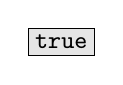
\begin{tikzpicture}
      \node [bddterminal] {$\true$};
    \end{tikzpicture}}
\newcommand{\bddfalse}[0]{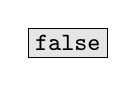
\begin{tikzpicture}
      \node [bddterminal] {$\false$};
    \end{tikzpicture}}


% Standardize command font styles and environments
\newcommand{\doccmd}[1]{\texttt{\textbackslash#1}}% command name -- adds backslash automatically
\newcommand{\docopt}[1]{\ensuremath{\langle}\textrm{\textit{#1}}\ensuremath{\rangle}}% optional command argument
\newcommand{\docarg}[1]{\textrm{\textit{#1}}}% (required) command argument
\newcommand{\docenv}[1]{\textsf{#1}}% environment name
\newcommand{\docpkg}[1]{\texttt{#1}}% package name
\newcommand{\doccls}[1]{\texttt{#1}}% document class name
\newcommand{\docclsopt}[1]{\texttt{#1}}% document class option name
\newenvironment{docspec}{\begin{quote}\noindent}{\end{quote}}% command specification environment



\begin{document}
\maketitle% this prints the handout title, author, and date
\begin{itemize}
  \item Note: not class next Tuesday, Sept 26 (Software Day)
  \item Join Slack, I make announcements there
\end{itemize}

\section{Binary decision diagrams (BDDs)}
\begin{itemize}
  \marginnote{BDDs were introduced by \citet{bryant1992symbolic}. \citet{meinel1998algorithms} is a 
  good reference for learning how to implement and analyze BDDs. \citet{knuth2013art} has a comprehensive 
  discussion on BDDs as well.}
  \item \textbf{Problem}: \prop$_S${} is not very expressive
  \item \textbf{Goal:} More expressive tractable languages
  \item What can we improve about \prop$_S$? Observe that there may be 
  \emph{repetitious sub-syntactic terms}, and we'd like to exploit those, just
  like we observed in our memoized reduction scheme
  \item How can we represent repetitious subterms syntactically? By changing our 
  syntax to permit \emph{directed acyclic graphs}!

  \item Syntax of \defn{binary decision diagrams} (BDDs):\marginnote{Here we give a BNF grammar that permits directed acyclic graphs as terms.
    This is quite non-standard: we are implicitly permitting the structural
    re-use of terms in this grammar, and assuming an induction principle that 
    ``inducts on the structure of DAGs'' in this definition of syntax. I don't
    want to get to into the weeds on this, so we will mostly see through examples how 
    we write terms in this language and perform proofs by structural induction.
    See \citet{braibant2014implementing} for some discussion on this.}
  \begin{align*}
    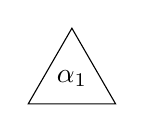
\begin{tikzpicture}
    \node [bddtriangle] {$\alpha_1$};
    \end{tikzpicture},
    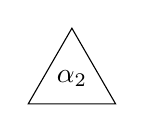
\begin{tikzpicture}
    \node [bddtriangle] {$\alpha_2$};
    \end{tikzpicture} :: = 
    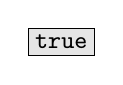
\begin{tikzpicture}
      \node [bddterminal] {$\true$};
    \end{tikzpicture} \mid 
    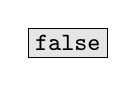
\begin{tikzpicture}
      \node [bddterminal] {$\false$};
    \end{tikzpicture} \mid
    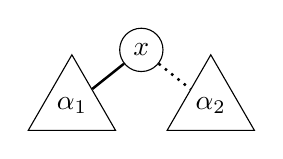
\begin{tikzpicture}
      \node (x) [bddnode] {$x$};
      \node (a1) at ($(x) + (-25bp, -20pt)$) [bddtriangle] {$\alpha_1$};
      \node (a2) at ($(x) + (25bp, -20pt)$) [bddtriangle] {$\alpha_2$};
    \begin{scope}[on background layer]
      \draw [highedge] (x) -- (a1);
      \draw [lowedge] (x) -- (a2);
    \end{scope}
    \end{tikzpicture}
  \end{align*}
  I.e., each BDD is a rooted directed acyclic graph with terminal nodes labeled 
  $\true$ and $\false$, and internal \emph{branch nodes} labeled by propositional 
  variables. The solid edge of a branch node is called the \emph{high edge}, and the 
  dashed edge is called the \emph{low edge}.
  \item Here are some example BDDs:

  \begin{figure}[h]
    \centering
    \begin{subfigure}[b]{0.4\textwidth}
  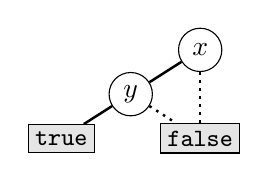
\begin{tikzpicture}
    \def\lvl{16pt}
    \node (x) at (0bp,0bp) [bddnode] {$x$};
    \node (y) at ($(x) + (-25bp, -\lvl)$) [bddnode] {$y$};
    \node (vt) at ($(y) + (-25bp, -\lvl)$) [bddterminal] {$\true$};
    \node (vf) at ($(y) + (25bp, -\lvl)$) [bddterminal] {$\false$};
    \begin{scope}[on background layer]
      \draw [highedge] (x) -- (y);
      \draw [lowedge] (x) -- (vf);
      \draw [lowedge] (y) -- (vf);
      \draw [highedge] (y) -- (vt);
    \end{scope}
  \end{tikzpicture}
  \caption{A BDD representing $x \land y$}
\end{subfigure}~~
\begin{subfigure}[b]{0.4\textwidth}
  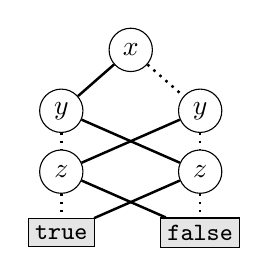
\begin{tikzpicture}
    \def\lvl{22pt}
    \node (x) at (0bp,0bp) [bddnode] {$x$};
    \node (y1) at ($(x) + (-25bp, -\lvl)$) [bddnode] {$y$};
    \node (y2) at ($(x) + (25bp, -\lvl)$) [bddnode] {$y$};
    \node (z1) at ($(y1) + (0, -\lvl)$) [bddnode] {$z$};
    \node (z2) at ($(y2) + (0, -\lvl)$) [bddnode] {$z$};
    \node (vt) at ($(z1) + (0, -\lvl)$) [bddterminal] {$\true$};
    \node (vf) at ($(z2) + (0, -\lvl)$) [bddterminal] {$\false$};
    \begin{scope}[on background layer]
      \draw [highedge] (x) -- (y1);
      \draw [lowedge] (x) -- (y2);
      \draw [lowedge] (y1) -- (z1);
      \draw [highedge] (y1) -- (z2);
      \draw [highedge] (y2) -- (z1);
      \draw [lowedge] (y2) -- (z2);
      \draw [lowedge] (z1) -- (vt);
      \draw [highedge] (z2) -- (vt);
      \draw [lowedge] (z2) -- (vf);
      \draw [highedge] (z1) -- (vf);
    \end{scope}
  \end{tikzpicture}
  \caption{A BDD representing $x \oplus y \oplus z$}
\end{subfigure}

\caption{Example \bdd{} programs.}
\end{figure}

  Solid edges are high edges, dotted edges are low edges. BDDs are read top-down, 
  where the implied directionality of the arrow is top-down.

  \item Observe that there can many equivalent ways of writing the same BDD for a 
  particular denotation (show examples on board)

  \item A BDD is called \emph{ordered} if each variable is used \emph{at most
  once} and in a \emph{fixed order}. We will consider only ordered BDDs.


  \item A BDD is called \emph{reduced} if, for every node 
  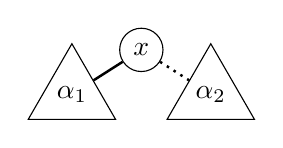
\begin{tikzpicture}
    \def\lvl{16pt}
    \node (x) at (0bp,0bp) [bddnode] {$x$};
    \node (t) at ($(x) + (-25bp, -\lvl)$) [bddtriangle] {$\alpha_1$};
    \node (f) at ($(x) + (25bp, -\lvl)$) [bddtriangle] {$\alpha_2$};
    \begin{scope}[on background layer]
      \draw [highedge] (x) -- (t);
      \draw [lowedge] (x) -- (f);
    \end{scope}
  \end{tikzpicture}, it is the case that $\bddtriangle{$\alpha_1$} \ne \bddtriangle{$\alpha_2$}$.
  \item We can enforce these constraints with a typing judgment that is reminescent of 
  \emph{ordered affine linear logic}~\citep{girard1987linear}.

  Let $\Gamma$ be an \emph{ordered} list of propositional variables.
  A term in \robdd{} is a \bdd{} term that satisfies the following typing judgment, written 
  $\Gamma \vdash \bddtriangle{}$:
  \begin{mathpar}
    \inferrule{}{\Gamma \vdash^r
      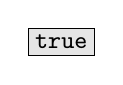
\begin{tikzpicture}
      \node [bddterminal] {$\true$};
      \end{tikzpicture}}
      \and 
    \inferrule{}{\Gamma \vdash^r
      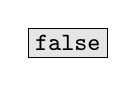
\begin{tikzpicture}
      \node [bddterminal] {$\false$};
      \end{tikzpicture}}
    \and 
    \inferrule*[Right=(\textsc{Weaken})]{\Gamma \vdash^r \bddtriangle{$\alpha$}}{x :: \Gamma \vdash^r \bddtriangle{$\alpha$}}
    \\
    \inferrule{\Gamma \vdash^r \bddtriangle{$\alpha_1$} \and \Gamma \vdash^r \bddtriangle{$\alpha_2$} \and 
    \bddtriangle{$\alpha_1$} \ne \bddtriangle{$\alpha_2$}
    }
    {x :: \Gamma \vdash^r 
        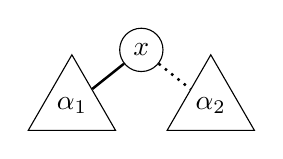
\begin{tikzpicture}
      \node (x) [bddnode] {$x$};
      \node (a1) at ($(x) + (-25bp, -20pt)$) [bddtriangle] {$\alpha_1$};
      \node (a2) at ($(x) + (25bp, -20pt)$) [bddtriangle] {$\alpha_2$};
    \begin{scope}[on background layer]
      \draw [highedge] (x) -- (a1);
      \draw [lowedge] (x) -- (a2);
    \end{scope}
    \end{tikzpicture}}
  \end{mathpar}


\begin{theorem}[Canonicity of ROBDD]
For two well-typed ROBDD terms $\Gamma \vdash^r \alpha_1$ and $\Gamma \vdash^r \alpha_2$,
it is the case that $\dbracket{\Gamma \vdash \alpha_1} =\dbracket{\Gamma \vdash \alpha_2}$ 
if and only if $\alpha_1 = \alpha_2$.
\end{theorem}
\begin{proof}
It is straightforward to show that if $\alpha_1 = \alpha_2$ then $\dbracket{\Gamma
\vdash^r \alpha_1} = \dbracket{\Gamma \vdash^r \alpha_2}$. The proof in the other 
direction follows by inducting on $|\Gamma|$. 

\textbf{Base case:} Assume $|\Gamma|$ = 0. Assume $\dbracket{\emptyset \vdash \alpha_1} = 
\dbracket{\emptyset \vdash \alpha_2}$. By our typing judgment for \robdd{},
$\alpha_1$ and $\alpha_2$ must each be either $\true$ or $\false$; these two cases 
have different semantics (either $\emptyset$ or $\{\top\}$), so we can conclude that this implies that $\alpha_1 = \alpha_2$.

\textbf{Inductive argument}: (come back if time, if no time, see
\citet{bryant1992symbolic} and \citet{knuth2013art} for an extended discussion)


% Assume $\dbracket{\Gamma \vdash^r \alpha_1} = \dbracket{\Gamma \vdash^r
% \alpha_2}$; we want to show that this implies that $\alpha_1 = \alpha_2$. The
% proof will proceed by induction on the size of 
% $\dbracket{\Gamma \vdash^r \alpha_1}$.

% \begin{itemize}
%   \item Base case: Assume $|\dbracket{\Gamma \vdash^r \alpha_1}| = 0$. 

%   We will show that $\alpha_1 = \false$ by induction on $\alpha_1$:

%   \begin{itemize}
%     \item   Base cases: If $\alpha_1 = \false$, we are done. If $\alpha_1 = \true$,
%       then $|\dbracket{\Gamma \vdash \true}| > 0$, which is a contradiction.
%     \item Inductive case: 
%   \end{itemize}


% \end{itemize}
\end{proof}





  \item We can enforce this ordering constraint with a typing judgment that is reminescent of 
  \emph{ordered affine linear logic}~\citep{girard1987linear}.

  Let $\Gamma$ be an \emph{ordered} list of propositional variables.
  A term in \robdd{} is a \bdd{} term that satisfies the following typing judgment, written 
  $\Gamma \vdash \bddtriangle{}$:
  \begin{mathpar}
    \inferrule{}{\Gamma \vdash
      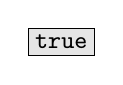
\begin{tikzpicture}
      \node [bddterminal] {$\true$};
      \end{tikzpicture}}
      \and 
    \inferrule{}{\Gamma \vdash
      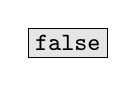
\begin{tikzpicture}
      \node [bddterminal] {$\false$};
      \end{tikzpicture}}
    \and 
    \inferrule*[Right=(\textsc{Weaken})]{\Gamma \vdash \bddtriangle{$\alpha$}}{x :: \Gamma \vdash \bddtriangle{$\alpha$}}
    \\
    \inferrule{\Gamma \vdash \bddtriangle{$\alpha_1$} \and \Gamma \vdash \bddtriangle{$\alpha_2$} \and 
    \bddtriangle{$\alpha_1$} \ne \bddtriangle{$\alpha_2$}
    }
    {x :: \Gamma \vdash 
        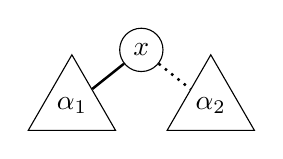
\begin{tikzpicture}
      \node (x) [bddnode] {$x$};
      \node (a1) at ($(x) + (-25bp, -20pt)$) [bddtriangle] {$\alpha_1$};
      \node (a2) at ($(x) + (25bp, -20pt)$) [bddtriangle] {$\alpha_2$};
    \begin{scope}[on background layer]
      \draw [highedge] (x) -- (a1);
      \draw [lowedge] (x) -- (a2);
    \end{scope}
    \end{tikzpicture}}
  \end{mathpar}

\

  \item Semantics of BDDs: Let $\Gamma$ be an ordered list of propositional variables. 
  For convenience, we define an operation $\otimes$ that adds an assignment to a set of instances, 
  i.e.:
  \begin{align*}
    &[x \mapsto \true] \otimes \{[z \mapsto \false], [z \mapsto \true]\} =\\ &\quad\quad \{[x \mapsto \true, z \mapsto \false], 
    [x \mapsto \true, z \mapsto \true]
    \}
  \end{align*}
  Formally, we say $[x \mapsto v] \otimes I = \{[x \mapsto v] \cup \gamma \mid \gamma \in I\}$.
  Then:
  \begin{align*}
    \dbracket{
    \Gamma \vdash 
      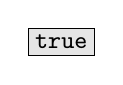
\begin{tikzpicture}
    \node (vt) [bddterminal] {$\true$};
    \end{tikzpicture}~} &= \dbracket{\Gamma}
    \\
    \dbracket{
    \Gamma \vdash 
      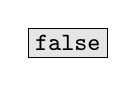
\begin{tikzpicture}
    \node (vt) [bddterminal] {$\false$};
    \end{tikzpicture}~} &= \emptyset
    \\
    \dbracket{
    x::\Gamma \vdash 
      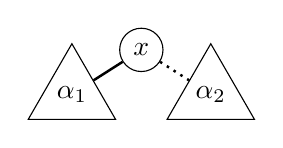
\begin{tikzpicture}
    \def\lvl{16pt}
    \node (x) at (0bp,0bp) [bddnode] {$x$};
    \node (t) at ($(x) + (-25bp, -\lvl)$) [bddtriangle] {$\alpha_1$};
    \node (f) at ($(x) + (25bp, -\lvl)$) [bddtriangle] {$\alpha_2$};
    \begin{scope}[on background layer]
      \draw [highedge] (x) -- (t);
      \draw [lowedge] (x) -- (f);
    \end{scope}
    \end{tikzpicture}~} &= 
    [x \mapsto \true] \otimes \dbracket{\Gamma \vdash \alpha_1} \cup
    [x \mapsto \false] \otimes \dbracket{\Gamma \vdash \alpha_2} \\
    \dbracket{
    y::\Gamma \vdash 
      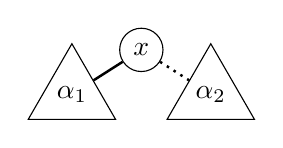
\begin{tikzpicture}
    \def\lvl{16pt}
    \node (x) at (0bp,0bp) [bddnode] {$x$};
    \node (t) at ($(x) + (-25bp, -\lvl)$) [bddtriangle] {$\alpha_1$};
    \node (f) at ($(x) + (25bp, -\lvl)$) [bddtriangle] {$\alpha_2$};
    \begin{scope}[on background layer]
      \draw [highedge] (x) -- (t);
      \draw [lowedge] (x) -- (f);
    \end{scope}
    \end{tikzpicture}~} &= 
    \dbracket{\Gamma \vdash 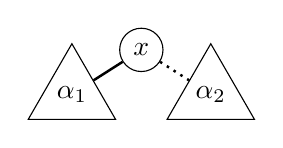
\begin{tikzpicture}
    \def\lvl{16pt}
    \node (x) at (0bp,0bp) [bddnode] {$x$};
    \node (t) at ($(x) + (-25bp, -\lvl)$) [bddtriangle] {$\alpha_1$};
    \node (f) at ($(x) + (25bp, -\lvl)$) [bddtriangle] {$\alpha_2$};
    \begin{scope}[on background layer]
      \draw [highedge] (x) -- (t);
      \draw [lowedge] (x) -- (f);
    \end{scope}
    \end{tikzpicture}
    }
  \end{align*}

We define $\dbracket{\Gamma}$ inductively:
\begin{align*}
  \dbracket{[]} &= \{\top\} \\
  \dbracket{x :: \Gamma} &= [x \mapsto \true] \otimes \dbracket{\Gamma} ~\bigcup~ 
    [x \mapsto \false] \otimes \dbracket{\Gamma}
\end{align*}
where $\top$ is the empty map.
\end{itemize}

\subsection{Probabilistic \bdd{}}
\begin{itemize}
  \item Just like how we made propositional logic, we can define a probabilistic
  version of BDDs and give them a probabilistic semantics. We call this language
  \bdd{}. 
  \item Syntax of \bdd{}: pairs $(\alpha, w)$, where $\alpha$ is a BDD and $w$
  is a map from propositional variables to probabilities
  \item The denotational semantics are nearly identical to \prop$_S${}, so we skip 
  then here. The operational semantic are quite similar as well:
  \begin{mathpar}
    \inferrule{}{(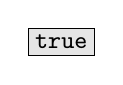
\begin{tikzpicture}
      \node [bddterminal] {$\true$};
    \end{tikzpicture}, w) \Downarrow 1}
    \and
    \inferrule{}{(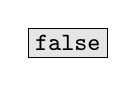
\begin{tikzpicture}
      \node [bddterminal] {$\false$};
    \end{tikzpicture}, w) \Downarrow 0} \\
    \inferrule{
      \bddtriangle{$\alpha_1$} \Downarrow v_1 \and \bddtriangle{$\alpha_2$} \Downarrow v_2
    }{
    \Big(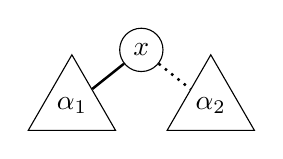
\begin{tikzpicture}
      \node (x) [bddnode] {$x$};
      \node (a1) at ($(x) + (-25bp, -20pt)$) [bddtriangle] {$\alpha_1$};
      \node (a2) at ($(x) + (25bp, -20pt)$) [bddtriangle] {$\alpha_2$};
    \begin{scope}[on background layer]
      \draw [highedge] (x) -- (a1);
      \draw [lowedge] (x) -- (a2);
    \end{scope}
    \end{tikzpicture}, w \Big) \Downarrow w(x) + v_1 + w(\overline{x})v_2}
  \end{mathpar}
  
  \item Is the above a a tractable runtime for \bdd{}? 
  This question is a bit subtle and depends on how we
  define structural induction on BDDs. For now, let's assume that we are caching as 
  traverse (just like the memoization routine from last time); this memoization routine 
  is a surely a tractable runtime for \bdd{}.
\end{itemize}

\begin{theorem}
  \bdd{} is more expressive than \prop$_S$.
\end{theorem}
\begin{proof}
  To show this, we must show two things: (1) that there is an efficient 
  compilation from \prop$_S$ to \bdd{}, and (2) that there is no efficient
  compilation from \bdd{} to \prop$_S$. Showing (1) is straightforward.
  Showing (2) is quite tricky.

  In general, there are the following strategies we can use to establish that there 
  is no efficient semantics-preserving translation:
  \begin{itemize}
    \item \emph{Denotational lower-bounds}: Show that there is a particular denotation
    that separates the two languages
    \item \emph{Reduction}: Show that the existence of a efficient
    semantics-preserving map can be used to give an efficient algorithm for something 
    we know is hard (i.e., solving SAT)
  \end{itemize}

In this case it is easier to give a denotational lower-bound\sidenote{...but,
if you can find a reduction, I'd be interested in seeing it!}.
We will have the following two lemmas that establish separation
between \prop$_S${} and \bdd{}:
\begin{lemma}
  For any integer $N$, There exists a BDD of size less than $2n$ whose
  denotation is equal to $\dbracket{\bigoplus_i^N x_i}$.
\end{lemma}
\begin{lemma}
  For any $N$ there does not exist a \prop$_S$ formula
  represents the denotation given by $\dbracket{\bigoplus_i^N x_i}$ 
  whose size is less than $2^N$.
\end{lemma}

\end{proof}

\subsection{Compiling \prop$_S$ to \bdd{}}
\marginnote{In the literature this process is typically called \emph{top-down 
knowledge compilation}. See \citep{darwiche2002knowledge,oztok2015top, darwiche2004new}.}
\begin{itemize}
  \item \textbf{Goal}: Build a compiler from \prop{} to \bdd{}. The weight function 
  translation is simple. We focus on translating formulae, which now has
  has a contextual compilation relation $(\pi, \varphi) \compiles \bdd{}$, where 
  now $\rho$ is a map from \prop{} to \bdd{}:

  \begin{mathpar}
    \inferrule{}{(\pi, \true) \compiles \bddtrue}
    \and
    \inferrule{}{(\pi, \false) \compiles \bddfalse}
    \and
    \\
    \inferrule{
      (\pi, \varphi[\true/x]) \compiles \bddtriangle{$\alpha_1$} \and \varphi[\false/x] \compiles \bddtriangle{$\alpha_2$}
      \and \bddtriangle{$\alpha_1$} \ne \bddtriangle{$\alpha_2$}
    }{
    \varphi \compiles
    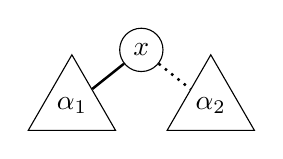
\begin{tikzpicture}
      \node (x) [bddnode] {$x$};
      \node (a1) at ($(x) + (-25bp, -20pt)$) [bddtriangle] {$\alpha_1$};
      \node (a2) at ($(x) + (25bp, -20pt)$) [bddtriangle] {$\alpha_2$};
    \begin{scope}[on background layer]
      \draw [highedge] (x) -- (a1);
      \draw [lowedge] (x) -- (a2);
    \end{scope}
    \end{tikzpicture}}
    \\
    \inferrule{
      \varphi[\true/x] \compiles \bddtriangle{$\alpha_1$} \and (\pi, \varphi[\false/x]) \compiles \bddtriangle{$\alpha_2$}
      \and \bddtriangle{$\alpha_1$} = \bddtriangle{$\alpha_2$}
    }{
    (x :: \pi, \varphi) \compiles \bddtriangle{$\alpha_1$}}

  \end{mathpar}
  
  \item \begin{theorem}
    The above compilation rule produces well-typed BDDs.
  \end{theorem}
  
  \item \textbf{Observe}: This looks almost identical to our memoized semantics
  $\Downarrow^m$. In some sense, the memoized semantics are efficient if and
  only if there exists a compilation to \bdd{}. This means that the syntax of
  \bdd{} perfectly captures the subset of \prop{} that can be executed
  efficiently by $\Downarrow^m$

  % \item Can we formalize this similarity? Here is an attempt:

  % \begin{conjecture}[Relative completeness of \bdd{} wrt. $\Downarrow^m$]
  %   Let \prog{} be a \prop{} program. Then, $\Downarrow^m$ is tractable in $|\prog|$ 
  %   if and only if there exists a semantics preserving translation from $\prog$ to 
  %   \bdd{}.
  % \end{conjecture}
\end{itemize}

\bibliographystyle{plainnat}
\bibliography{../bib}


\end{document}